\section{\'Ecriture et lecture des nombres en base 10}

% remarque : pour qu'un mot se retrouve dans le lexique : \MotDefinition{asymptote horizontale}{} 

Les règles et conventions qui permettent d'écrire et de lire les nombres forment ce qu'on appelle un \textbf{système de numération}. Nous utilisons le système décimal, de base dix.

\begin{aconnaitre}
Pour écrire les chiffres dans le système décimal, il nous faut dix symboles, appelés des \emph{chiffres}. Ces chiffres sont :
\[ 0\,;\,1\,;\,2\,;\,3\,;\,4\,;\,5\,;\,6\,;\,7\,;\,8\,;\,9  \]
Il arrive parfois qu'on confonde \textbf{\MotDefinition{chiffre}{}} et \textbf{\MotDefinition{nombre}{}}. On peut faire l'analogie avec l'écriture d'une langue en affirmant que les \textbf{chiffres} sont des \textbf{lettres} et que les \textbf{nombres} sont des \textbf{mots}. Ainsi, 13 est un nombre qui s'écrit avec les chiffres 1 et 3.
\end{aconnaitre}

\vspace{2em}

L'\textbf{écriture décimale} d'un nombre comporte deux parties, séparées par une virgule :

\hspace{2em}\textbullet\hspace{.25em} la partie entière, à gauche de la virgule ;

\hspace{2em}\textbullet\hspace{.25em} la partie décimale, à droite de la virgule.



Un nombre entier est caractérisé par le fait qu'il n'a pas de parti décimale (on omet alors la virgule).
% Il manque le tableau !
\begin{exemple*1}
\begin{itemize}
 \item Le premier nombre figurant dans le tableau s'écrit 3\,027\,462.\\
Il se lit "trois millions vingt-sept mille quatre cent soixante-deux".\\
C'est un nombre entier.\\
 \item Le  deuxième nombre figurant dans le tableau s’écrit 10,01.\\
Il se lit "dix virgule zéro un".\\
Ce n’est pas un nombre entier.\\
 \item Le troisième nombre figurant dans le tableau s’écrit 0,037.\\
Il se lit "zéro virgule zéro trente-sept" ou "trente-sept millièmes".\\
Ce n’est pas un nombre entier.\\
 \item Le quatrième nombre figurant dans le tableau s’écrit 20\,000\,042\,000.\\
Il se lit "vingt milliards quarante-deux mille".\\
C’est un nombre entier.\\
 \end{itemize}
\end{exemple*1}

\vspace{1em}{\large\textcolor{B1}{\textbf{Exercice << À toi de jouer >>}}}

Donne une écriture décimale du nombre cinquante-trois millions quatre cent vingt-sept mille huit cent dix-neuf virgule zéro zéro cinq cent soixante-et-un.

%%%%%%%%%%%%%%%%%%%%%%%%%%%%%%%%%%%%%%%%%%%%%%%%%%%%%%%%%%%%%%%%%%%%%%%%%%%

\section{Repérer sur une demi-droite graduée}

\begin{aconnaitre}
Sur une demi-droite graduée, un point est repéré par un nombre appelé son \textbf{\MotDefinition{abscisse}{}}.
\end{aconnaitre}

\begin{exemple*1}

 \begin{minipage}[c]{.46\textwidth}
 Donne l'abscisse des points $A$ et $B$ puis place le point $C$ d'abscisse 4,3.
  \end{minipage}\hfill%
 \begin{minipage}[c]{.46\textwidth} 
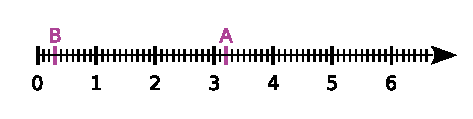
\includegraphics[width=\linewidth]{axe0BA6}
 \end{minipage}\\

Une unité est divisée en dix parts égales, ce qui signifie qu'elle est partagée en dix dixièmes. Le point $A$ se trouve 2 dixièmes à la droite du 3, donc son abscisse est $3 + 0,2 = 3,2$. De la même façon, $B$ a pour abscisse $0 + 0,3 = 0,3$. \\

  \begin{minipage}[c]{.46\textwidth}
On note $A(3,2)$ et $B(0,3)$.\\
$C(4,3) : 4,3 = 4 + 0,3$\\
$C$ se place 3 dixièmes à la droite du 4.
  \end{minipage}\hfill%
 \begin{minipage}[c]{.46\textwidth} 
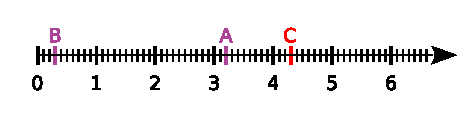
\includegraphics[width=\linewidth]{axe0BAC6}
 \end{minipage}\\

\end{exemple*1}

\vspace{1em}{\large\textcolor{B1}{\textbf{Exercice << À toi de jouer >>}}}

Sur une demi-droite graduée, place les points $M$ d'abscisse 2,7 et $N$ d'abscisse 5,2.
%%%%%%%%%%%%%%%%%%%%%%%%%%%%%%%%%%%%%%%%%%%%%%%%%%%%%%%%%%%%%%%%%%%%%%%%%%%
\section{Encadrer}

\begin{aconnaitre}
\textbf{\MotDefinition{Encadrer}{}} un nombre, c'est trouver un nombre qui est plus petit que lui et un nombre qui est plus grand que lui. On écrit un encadrement avec les symboles $<$ ; $\leqslant$ ; $>$ et $\geqslant$. 
\end{aconnaitre}

\begin{exemple*1}
Encadrer 13,345 à l'unité puis au centième.\\[1em]

Pour encadrer à l'unité, on «coupe» le nombre 13,345 à l'unité et on obtient 13 qui est plus petit  que 13,345. Puis on ajoute \textbf{une unité}. On obtient 14 qui est plus grand que 13,345. On écrit alors : $13 < 13,345 < 14$.


Pour encadrer au centième, on «coupe» le nombre 13,345 au centième et on obtient 13,34 qui est plus petit que 13,345. Puis on ajoute \textbf{un centième}. On obtient 13,35 qui est plus grand que 13,345. On écrit alors : $13,34 < 13,345 < 13,35$.
\end{exemple*1}

\vspace{1em}{\large\textcolor{B1}{\textbf{Exercice << À toi de jouer >>}}}

Encadrer les nombres 237,48 et 43,9235 à la dizaine puis au centième.
%%%%%%%%%%%%%%%%%%%%%%%%%%%%%%%%%%%%%%%%%%%%%%%%%%%%%%%%%%%%%%%%%%%%%%%%%%

\section{Arrondir}

\begin{aconnaitre}
\textbf{\MotDefinition{Arrondir}{}} un nombre, c’est le remplacer par le nombre le plus proche à la précision désirée. Pour cela, on choisit le dernier chiffre à conserver puis :
\begin{itemize}
 \item on conserve ce chiffre si le suivant est 0, 1, 2, 3 ou 4 ;
 \item on augmente de 1 ce chiffre si le suivant est 5, 6, 7, 8, ou 9.
 \end{itemize}
\end{aconnaitre}

%%%%%%%%%%%%%%%%%%%%%%%%%%%%%%%%%%%%%%%%%%%%%%%%%%%%%%%%%%%%%%%%%%%%%%%%%%

\section{Multiplier ou diviser un nombre décimal par 10 ; 100 ; 1\,000 \ldots}

\begin{aconnaitre}
\textbf{Multiplier} un nombre décimal par \textcolor{A1}{\textbf{10}}, \textcolor{B1}{\textbf{100}} ou \textcolor{J1}{\textbf{1\,000}} revient à déplacer chacun de ses chiffres vers \textbf{la gauche} de \textcolor{A1}{\textbf{1}}, \textcolor{B1}{\textbf{2}} ou \textcolor{J1}{\textbf{3}} rangs pour lui donner une valeur \textcolor{A1}{\textbf{10}}, \textcolor{B1}{\textbf{100}} ou \textcolor{J1}{\textbf{1\,000}} fois plus grande.
\textbf{Diviser} un nombre décimal par \textcolor{A1}{\textbf{10}}, \textcolor{B1}{\textbf{100}} ou \textcolor{J1}{\textbf{1\,000}} revient à déplacer chacun de ses chiffres vers \textbf{la droite} de \textcolor{A1}{\textbf{1}}, \textcolor{B1}{\textbf{2}} ou \textcolor{J1}{\textbf{3}} rangs pour lui donner une valeur  \textcolor{A1}{\textbf{10}}, \textcolor{B1}{\textbf{100}} ou \textcolor{J1}{\textbf{1\,000}} fois plus petite.
\end{aconnaitre}

\begin{remarque}
On devra parfois ajouter des zéros dans l'écriture.
\end{remarque}

\begin{exemple*1}
Effectue les calculs 6,5100 et $0,47 \cdot 1\,000$.\\[1em] % Il manque ici un tableau avec texte accordé en couleur
Pour diviser 6,5 par \textcolor{B1}{\textbf{100}}, on déplace chacun de ses chiffres vers la droite de \textcolor{B1}{\textbf{2}} rangs et on ajoute les zéros nécessaires. 

On obtient $6,5100 = 0,065$.

Pour multiplier 0,47 par \textcolor{J1}{\textbf{1\,000}}, on déplace chacun de ses chiffres vers la gauche de \textcolor{J1}{\textbf{3}} rangs et on ajoute les zéros nécessaires. 

On obtient $0,47 \cdot 1\,000 = 470$. 

\end{exemple*1}

\vspace{1em}{\large\textcolor{B1}{\textbf{Exercice << À toi de jouer >>}}}

Effectue : a) $3,6 \cdot 100$ \hfill b) $870 \cdot 1\,000$ \hfill  c) $63 : 10$ \hfill d) $87\,654 : 100$
 
Convertis en cm : a) 4 dm \hfill b) 8,1 dam \hfill c) 3,5 mm \hfill d) 0,035 m

%%%%%%%%%%%%%%%%%%%%%%%%%%%%%%%%%%%%%%%%%%%%%%%%%%%%%%%%%%%%%%%%%%%%%%%%%%%

\section{Multiplier ou diviser un nombre décimal par 0,1 ; 0,01 ; 0,001 \ldots}

\begin{aconnaitre}
\textbf{Multiplier} un nombre décimal par \textcolor{A1}{\textbf{0,1}}, \textcolor{B1}{\textbf{0,01}} ou \textcolor{J1}{\textbf{0,001}} revient à déplacer chacun de ses chiffres vers \textbf{la droite} de 1, 2 ou \textcolor{J1}{\textbf{3}} rangs pour lui donner une valeur 10, 100 ou \textcolor{J1}{\textbf{1\,000}} fois plus petite.
\textbf{Diviser} un nombre décimal par \textcolor{A1}{\textbf{0,1}}, \textcolor{B1}{\textbf{0,01}} ou \textcolor{J1}{\textbf{0,001}} revient à déplacer chacun de ses chiffres vers \textbf{la gauche} de \textcolor{A1}{\textbf{1}}, \textcolor{B1}{\textbf{2}} ou \textcolor{J1}{\textbf{3}} rangs pour lui donner une valeur \textcolor{A1}{\textbf{10}}, \textcolor{B1}{\textbf{100}} ou \textcolor{J1}{\textbf{1\,000}} fois plus grande.
\end{aconnaitre}

\begin{remarque}
On devra parfois ajouter des zéros dans l'écriture.
\end{remarque}

\begin{exemple*1}
Effectue les calculs $2,5 \times 0,01$ et $0,65 \div 0,001$.\\[1em]
% Il manque un tableau. Les chiffres 10, 100 et 1000 doivent être en couler accordée avec l'image qui suit.
Pour multiplier 2,5 par \textcolor{B1}{\textbf{0,01}}, on déplace chacun de ses chiffres vers la droite de \textcolor{B1}{\textbf{2}} rangs et on ajoute les zéros nécessaires. 

On obtient $2,5 \times 0,01 = 0,025$.

Pour diviser 0,65 par \textcolor{J1}{\textbf{0,001}}, on déplace chacun de ses chiffres vers la gauche de \textcolor{J1}{\textbf{3}} rangs et on ajoute les zéros nécessaires. 

On obtient $0,65 \div 0,001 = 650$. 
\end{exemple*1}

\vspace{1em}{\large\textcolor{B1}{\textbf{Exercice << À toi de jouer >>}}}

Effectuer : a) $5,45 \cdot 0,1$ \hfill b) $854 \cdot 0,001$ \hfill c) $63 \div 0,1$ \hfill d) $87,54 \div 0,01$
%%%%%%%%%%%%%%%%%%%%%%%%%%%%%%%%%%%%%%%%%%%%%%%%%%%%%%%%%%%%%%%%%%%%%%%%%%%

\section{Multiplier deux nombres décimaux}

\begin{exemple*1}
Effectue la multiplication de 2,34 par 1,2.\\[1em]

On pose l'opération comme s'il s'agissait de nombres entiers. 

On effectue la multiplication de 234 par 12 sans tenir compte des virgules.\\[0.75em]
234 est \textcolor{B1}{\textbf{100}} fois plus grand que 2,34 et 12 est 10 fois plus grand que 1,2. Le produit $2,34 \cdot 1,2$ est donc \textcolor{J1}{\textbf{1\,000}} fois plus petit que 2\,808. Pour obtenir le résultat, on effectue donc $2\,808 : 1\,000$.\\[0.75em]
Finalement $2,34 \cdot 1,2 = 2,808$.
% Il manque un tableau. Mettre les couleurs aux chiffres du tableau.
\end{exemple*1}

\vspace{1em}{\large\textcolor{B1}{\textbf{Exercice << À toi de jouer >>}}}

Sachant que $168 \cdot 32 = 5\,376$, détermine les produits (sans aucun calcul) :

a) $168 \cdot 3,2$ \hfill b) $16,8 \cdot 0,32$ \hfill  c) $1\,680 \cdot 3,2$ \hfill d) $1,68 \cdot 32$

Pose et effectue les opérations :

a) $68,7 \cdot 39$ \hfill b) $123 \cdot 6,3$ \hfill c) $1,3 \cdot 0,7$ \hfill d) $54,6 \cdot 8,25$
%%%%%%%%%%%%%%%%%%%%%%%%%%%%%%%%%%%%%%%%%%%%%%%%%%%%%%%%%%%%%%%%%%%%%%%%%%%    

\section{Diviser un nombre décimal par un nombre entier}

\begin{exemple*1}
Effectue la division de 75,8 par 4.\\[1em]

\begin{minipage}[c]{.26\textwidth}
\vspace{0em}
\begin{center}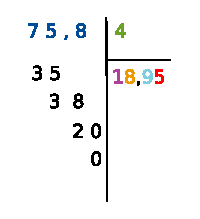
\includegraphics[width=3cm]{div758-4} \end{center}

\end{minipage}\hfill% 
\begin{minipage}[c]{.66\textwidth}

On commence par diviser la partie entière. On partage \textcolor{A1}{7} dizaines en \textcolor{H1}{4} ; le quotient comportera \textcolor{C1}{1} dizaine.\\[0.75em]
Il reste 3 dizaines. Avec les \textcolor{A1}{5} unités en plus, cela fait 35 unités à partager en \textcolor{H1}{4} ; le quotient comportera \textcolor{J1}{8} unités. \\[0.75em]
Il reste 3 unités soit 30 dixièmes. Avec les \textcolor{A1}{8} dixièmes en plus, cela fait 38 dixièmes à partager en \textcolor{H1}{4} ; le quotient comportera \textcolor{A3}{9} dixièmes. On doit donc écrire la virgule dans le quotient.\\[0.75em]
Il reste 2 dixièmes soit 20 centièmes (on a ajouté un zéro) à partager en \textcolor{H1}{4} ; le quotient comportera donc \textcolor{B2}{5} centièmes.\\[0.75em]
Ainsi $\textcolor{A1}{75,8} : \textcolor{H1}{4} = \textcolor{C1}{1}\textcolor{J1}{8},\textcolor{A3}{9}\textcolor{B2}{5}$.
\end{minipage}

\end{exemple*1}

\vspace{1em}{\large\textcolor{B1}{\textbf{Exercice << À toi de jouer >>}}}

Calcule la valeur exacte ou une valeur arrondie au centième des quotients :

a) $10 : 7$ \hfill  b) $24,96 : 8$ \hfill c) $5,2 : 6$ \hfill d) $145,2 : 3$
%%%%%%%%%%%%%%%%%%%%%%%%%%%%%%%%%%%%%%%%%%%%%%%%%%%%%%%%%%%%%%%%%%%%%%%%%%%

\section{Diviser un nombre décimal par un nombre décimal}

\begin{aconnaitre}
Le quotient de deux nombres \textbf{ne change pas} si on les multiplie (le dividende et le diviseur) par un même nombre non nul.
\end{aconnaitre}

\begin{exemple*1}
Effectue la division de 32,4 par 2,25.\\[1em]

On commence par rendre entier le diviseur en le multipliant par 100 : $2,25 \cdot 100 = 225$. On multiplie le dividende par le même nombre : $32,4 \cdot 100 = 3\,240$. On effectue la division de 3\,240  par 226, soit $3\,240 : 225 = 14,4$. On obtient ainsi le résultat de la division :

$32,4 : 2,25 = 14,4$. 
\end{exemple*1}

\vspace{1em}{\large\textcolor{B1}{\textbf{Exercice << À toi de jouer >>}}}

Calcule la valeur exacte ou une valeur arrondie au centième des quotients :

a) $4 : 6,37$ \hfill b) $13,4 : 2,45$ \hfill c) $5,87 : 2,3$ \hfill d) $0,84 : 0,12$
%%%%%%%%%%%%%%%%%%%%%%%%%%%%%%%%%%%%%%%%%%%%%%%%%%%%%%%%%%%%%%%%%%%%%%%%%%%        

\section{Opérations sur les durées} 

\subsection{Conversion en minutes ou en secondes}

\begin{exemple*1}
\begin{enumerate}
 \item Combien y a-t-il de minutes dans 5 h 27 min ?
 \item Combien y a-t-il de secondes dans 2 h 47 min 53 s ?
 \end{enumerate}
 




\begin{enumerate}
 
 \item \emph{Correction}

\begin{tabular}{lcl} 
\textcolor{bleu}{\textbf{5 h}} $=$ \textcolor{bleu}{\textbf{5}} $\times$ 60 min $=$ \textcolor{bleu}{\textbf{300 min}}  & $\longrightarrow$ & On convertit les heures en minutes. \\
\textcolor{bleu}{\textbf{5 h}} \textcolor{vert}{\textbf{27 min}} $=$ \textcolor{bleu}{\textbf{300 min}} $+$ \textcolor{vert}{\textbf{27 min}} $=$ 327 min & $\longrightarrow$ & On termine le calcul.\\
\phantom{2 h 47 min 53 s $=$ 7\,200 s $+$ 2\,820 s $+$ 53 s $=$ 10\,073 s} & \\ % phantom pour alignement avec tableau ci-dessous
 \end{tabular} 
 
 \item \emph{Correction}
 
\begin{tabular}{lcl} 
\textcolor{bleu}{\textbf{2 h}} $=$ \textcolor{bleu}{\textbf{2}} $\times$ 3\,600 s $=$ \textcolor{bleu}{\textbf{7\,200 s}} & $\longrightarrow$ & On convertit les heures en secondes. \\
\textcolor{vert}{\textbf{47 min}} $=$ \textcolor{vert}{\textbf{47}} $\times$ 60 s $=$ \textcolor{vert}{\textbf{2\,820}} s & $\longrightarrow$ & On convertit les minutes en secondes. \\
\textcolor{bleu}{\textbf{2 h}} \textcolor{vert}{\textbf{47 min}} 53 s $=$ \textcolor{bleu}{\textbf{7\,200 s}} $+$ \textcolor{vert}{\textbf{2\,820}} s $+$ 53 s $=$ 10\,073 s & $\longrightarrow$ & On termine le calcul. \\
 \end{tabular}
 \end{enumerate}
\end{exemple*1}

\subsection{Conversion en heures, minutes et secondes}

\begin{exemple*1}
Combien y a-t-il d'heures, minutes et secondes dans 41\,000 s ? \\[1em]



\begin{minipage}[t]{.46\textwidth}
On convertit les secondes en minutes et secondes en posant la division de 41\,000 par 60.

\begin{center}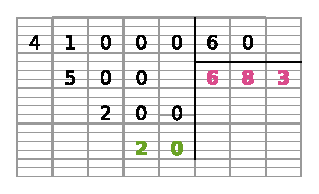
\includegraphics[width=4.6cm]{41000div60}

On a donc 41\,000 s $=$ \textcolor{rose}{\textbf{683 min}} \textcolor{vert}{\textbf{20 s}}.\end{center}
\end{minipage}\hfill%
\begin{minipage}[t]{.46\textwidth}
On convertit alors les minutes en heures et minutes en effectuant la division euclidienne de 683 par 60.

\begin{center}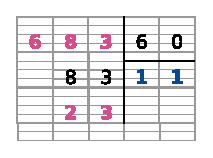
\includegraphics[width=2.9cm]{683div60}

On a donc 41\,000 s $=$ \textcolor{bleu}{\textbf{11 h}} \textcolor{rose}{\textbf{23 min}} \textcolor{vert}{\textbf{20 s}}.\end{center}
\end{minipage}



\end{exemple*1}

\subsection{Addition de durées}

\begin{exemple*1}
Un match dure 3 h 38 min et le suivant dure 2 h 49 min. Quelle est la durée totale de ces deux matchs ? \\[1em]



\begin{minipage}[t]{.34\textwidth}
On pose l'addition suivante.\\[0.2em]

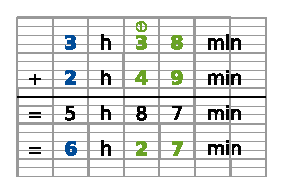
\includegraphics[width=\linewidth]{grille3h38}
\end{minipage}\hfill%
\begin{minipage}[t]{.60\textwidth}
On effectue deux additions indépendantes : 
\textcolor{vert}{\textbf{les minutes entre elles}} et \textcolor{bleu}{\textbf{les heures entre elles}}.\\[0.75em]
Mais le nombre de minutes obtenu est supérieur à 59. 
On va donc le convertir en heures et minutes sachant que 60 min $=$ 1 h. \\[0.75em]
La durée totale de ces deux matchs est donc de \textcolor{rose}{\textbf{6 h 27 min}}.
\end{minipage}

\end{exemple*1}

\subsection{Soustraction de durées}

\begin{exemple*1}
Un film débute à 15 h 27 et finit à 18 h 14. Quelle est la durée de ce film ? \\[1em]



\begin{minipage}[t]{.34\textwidth}
On pose la soustraction suivante.\\[0.2em]

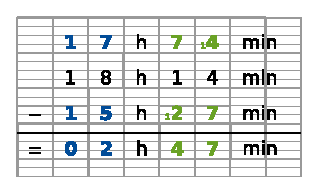
\includegraphics[width=\linewidth]{grille17h74}
\end{minipage}\hfill%
\begin{minipage}[t]{.60\textwidth}
On effectue deux soustractions indépendantes : 
\textcolor{vert}{\textbf{les minutes entre elles}} et \textcolor{bleu}{\textbf{les heures entre elles}}.\\[0.75em]
Mais on ne peut pas enlever 27 à 14. 
On va donc convertir 1 des 18 heures en 60 min. \\[0.75em]
Ce film dure donc \textcolor{rose}{\textbf{2 h 47 min}}.
\end{minipage}

\end{exemple*1}

\vspace{1em}{\large\textcolor{B1}{\textbf{Exercice << À toi de jouer >>}}}

Calcule : 3 h 05 min 13 s $+$ 56 min 48 s puis 1 h 35 min 29 s $-$ 46 min 37 s.

Calcule : 1 h 46 min $+$ 2 h 37 min et 9 min 16 s $-$ 7 min 55 s.